    \subsubsection[Fix]{Sole fisso}
        \begin{frame}{NOTA - Simulazioni con sole fermo}
            \begin{columns}
                \column{.5\textwidth}
                    \centering
                    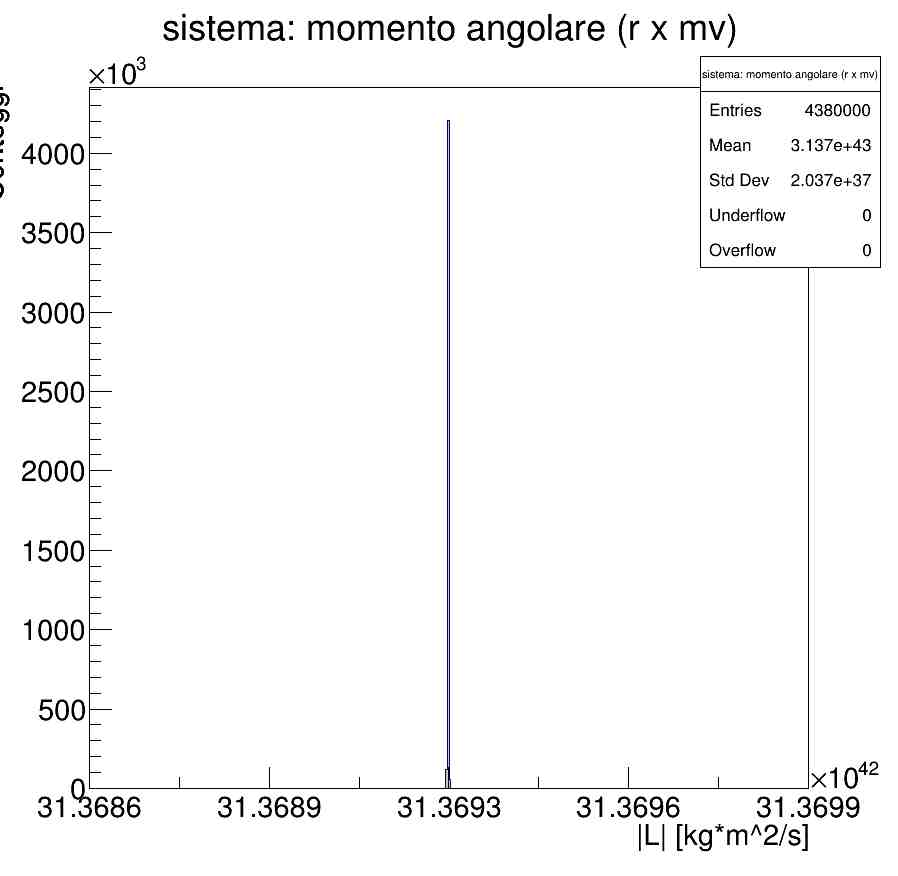
\includegraphics[width=\textwidth, height=3.75cm]{14_fisso/sf_Ltot.jpg}\\
                    \includegraphics[width=\textwidth, height=3.75cm]{14_fisso/.jpg}
                    %metti grafico eccentricità
                \column{.5\textwidth}
                    \centering
                    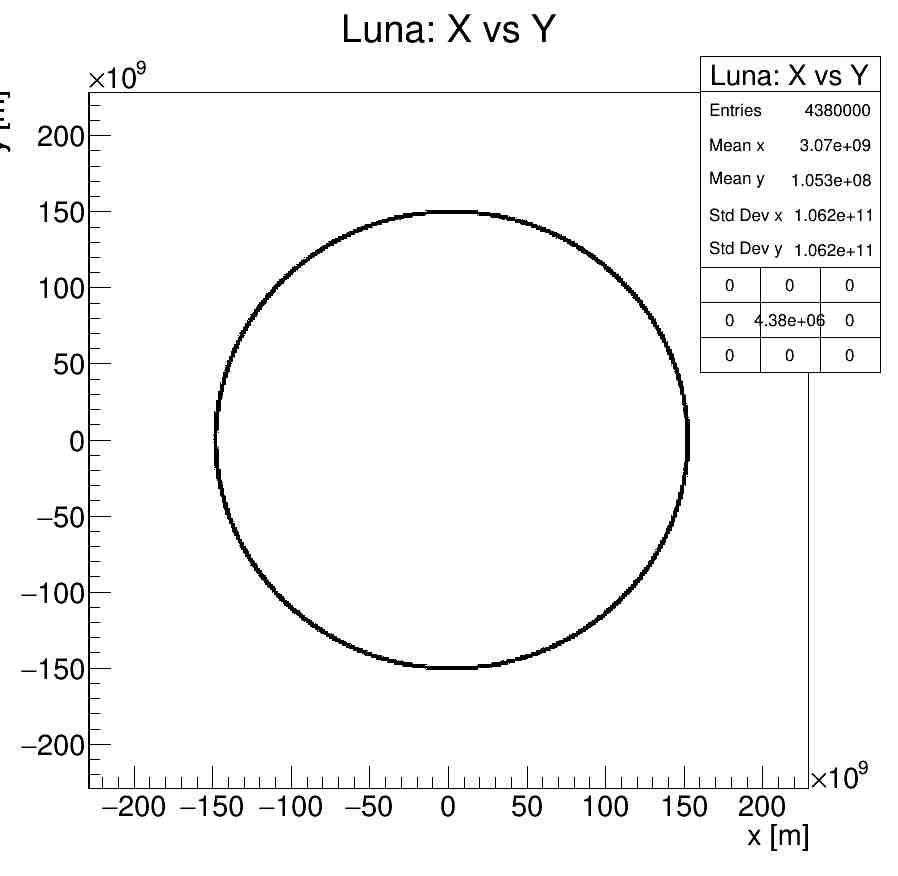
\includegraphics[width=\textwidth]{14_fisso/sf_terra_ok.jpg}\\\
                    \includegraphics[width=\textwidth]{}     
            \end{columns}
        \end{frame}
        \begin{frame}{NOTA - Simulazioni con sole fermo}
            Deriva per tempi lunghi
            \vspace{1cm}
            \begin{columns}
                \column{.5\textwidth}
                    \centering
                    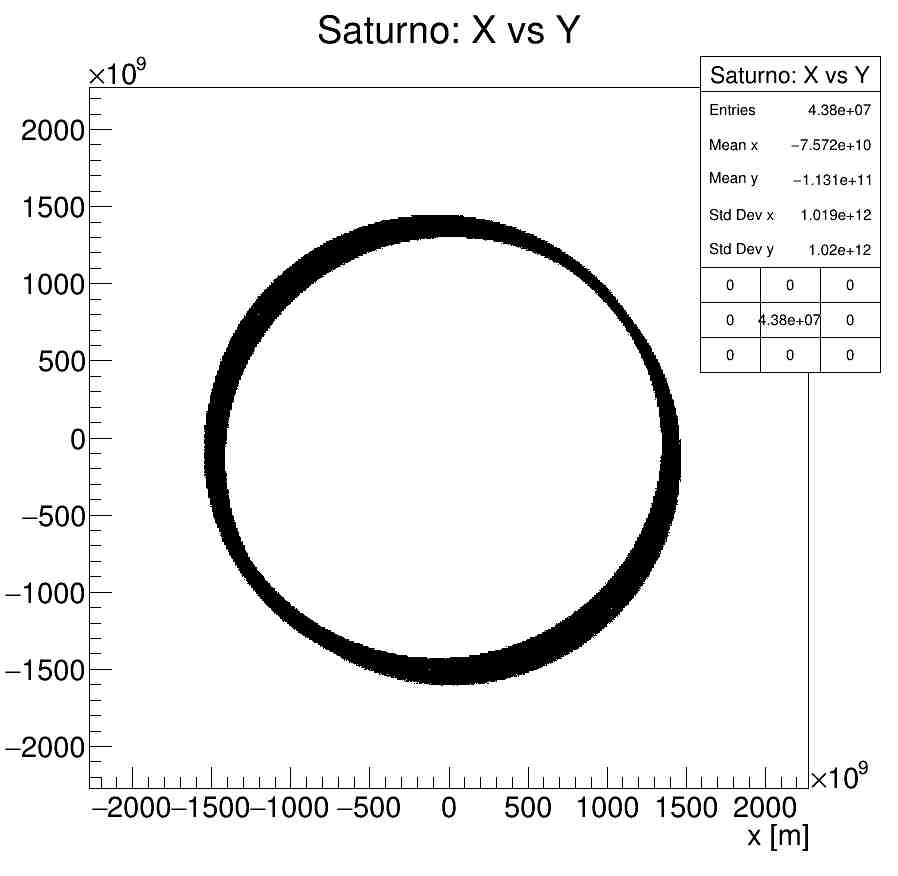
\includegraphics[width=\textwidth]{14_fisso/sf_5k_sat_orb.jpg}  
                \column{.5\textwidth}
                    \centering
                    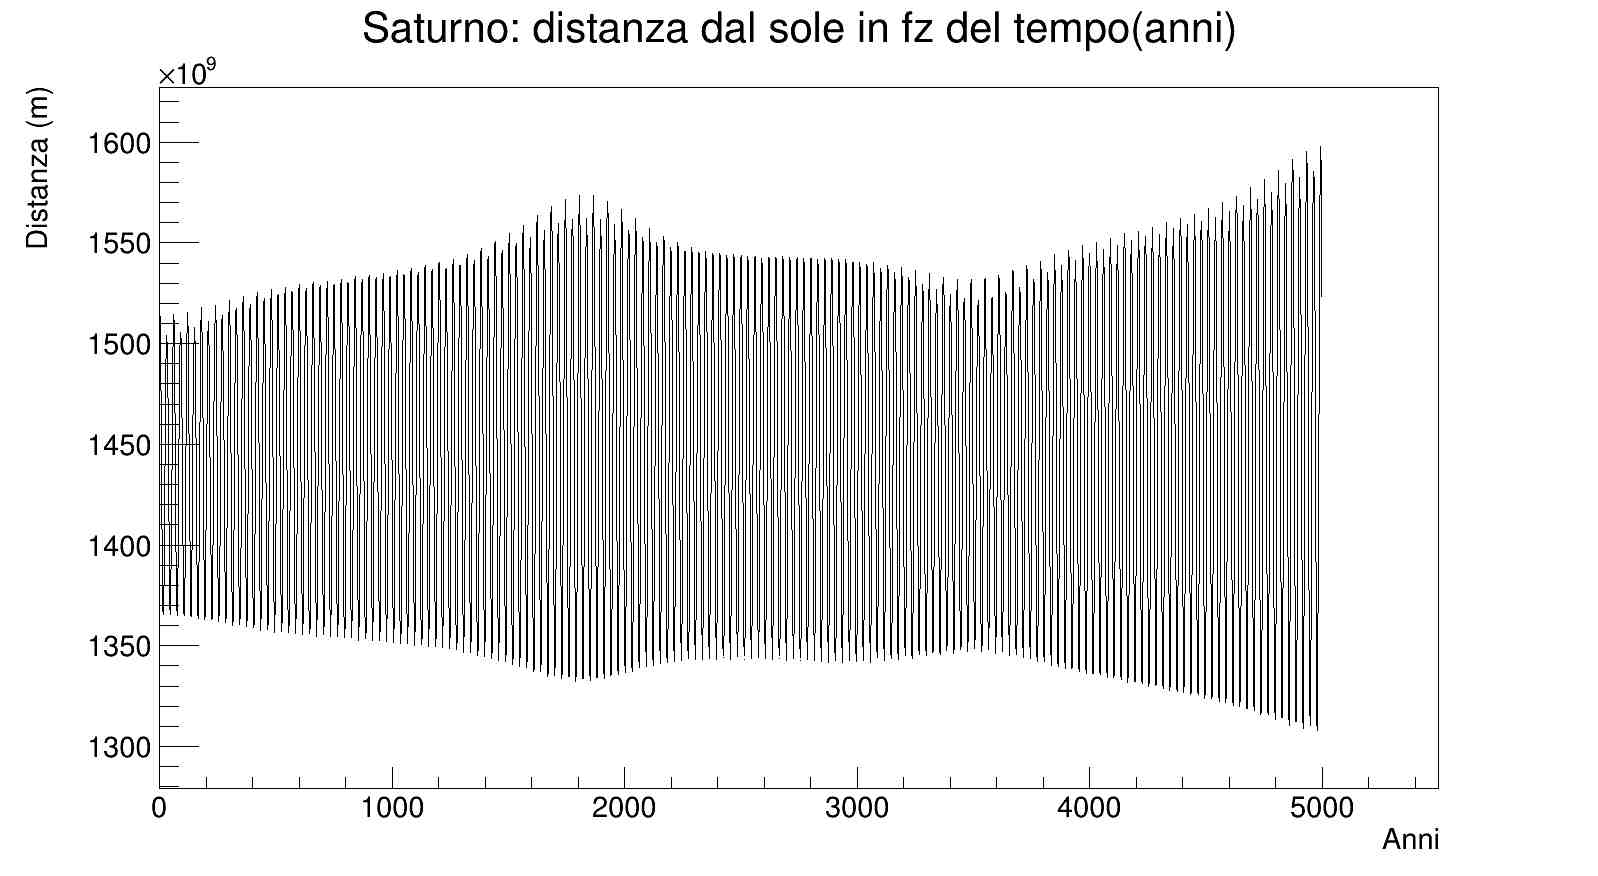
\includegraphics[width=\textwidth]{14_fisso/sf_5k_sat_drift.jpg}   
            \end{columns}
        \end{frame}